\chapter{Umsetzung}
Dieses Kapitel erläutert alle Schritte der Umsetzung des GuttenBase Plugins beginnend mit der Analyse bis zu zur Architektur und Implementierung.
\section{Analyse}
Am Anfang dieses Abschnitts wird die Umsetzungsform des GuttenBase Plugins festgelegt, da diese einen Einfluss auf die Architektur sowie die zu verwendenen Technologien hat. Außerdem werden die Anforderungen an das System definiert.\\
Um den Soll-Zustand genauer zu definieren werden Prototypen eingesetzt.
\subsection{Umsetzungsform}
Um eine optimale Nutzung des GuttenBase Plugins zu erzielen, soll auf die Umsetzungsform geachtet werden.\\
Das zu entwickelnde Tool kann z. B. als eine Desktop Applikation, Web Applikation oder als Plugin einer anderen Anwendung realisiert werden.\\
In der Tabelle \ref{table:tool-options} werden einige Vor- und Nachteie jeder Alternative erläutert. \\
Alle drei Alternativen haben Pros und Contras allerdings ist die schnellere Erreichung von vielen Nutzern sowie die Einfache Installation bei der IDE Plugin Entwicklung entscheidend. 
\begin{table}
	\centering
		\begin{tabular}{ |p{3cm}|p{6cm}|p{6cm}| }
			\hline
			\textbf{Alternative} & \textbf{Vorteile} &  \textbf{Nachteile}  \\
			Desktop App & 
			\begin{itemize}
				\item Offline immer verfügbar
				\item Volle Kontrolle über die Anwendung und die enthaltenen Daten.
				\item Bessere Leistung, da kein Browser als Zwischenschicht existiert.
			\end{itemize}& 
			\begin{itemize}
				\item Platformabhängig
				\item Hohe Entwicklungskosten
				\item Installation ist notwendig
			\end{itemize} \\
			\hline
			Web App &
			
			\begin{itemize}
				\item Installation oder manuelle Updates sind nicht notwändig. 
				\item geringere Entwicklung- und Wartungskosen, da die Anwendung unabhängig von lokalen Endgeräten ist.
			\end{itemize} &
		
			\begin{itemize}
				\item Offline meistens nicht verfügbar.
				\item Geringere Leistung.
				\item Es kann auf bestimmte Gerätehardware nicht zugegriffen werden.
			\end{itemize} \\
			\hline
			IDE Plugin Entwicklung &
			
			\begin{itemize}
				\item Viele Nutzer können erreicht werden.
				\item Einfach zu installieren.
				\item Manche Komponenten bzw. Funktionalitäten der zu erweiternden IDE können wiederverwwendet werden, was die Entwicklungsdauer verkürzt.
				\item Intuitive Nutzung sowie eine einheitliche Benutzeroberfläche wie die benutzte IDE.
			\end{itemize} &
			
			\begin{itemize}
				\item Einarbeitung in die Plugin Entwicklung der ausgewählten IDE ist erforderlich.
				\item Die Flexibilität beim Entwickeln ist durch die limitierte Erweiterbarkeit der IDE eingeschränkt.
			\end{itemize} \\
			\hline
		
		\end{tabular}
	\caption{Umsetzungsmöglichkeiten}
	\label{table:tool-options}
\end{table}

Zunächst soll für eine konkrete IDE entschieden werden. Um diese auszuwählen, muss auf die Anzahl der Nutzer, die Verfügbarkeit der Dokumentation für Plugin Entwicklung sowie die Unterstützung von Datenbanken geachtet werden.\\
Einer der bekanntesten Methoden, um die Beliebtheit einer Programmiersprache bzw. eine IDE herauszufinden, ist der PYPL-Index. Er basiert sich auf Rohdaten aus Google Trends. PYPL enthält den TOP-IDE-Index, welches alanysiert, wie oft IDEs bei Google durchgesucht werden. Die Suchanfragen spiegeln zwar nicht unbedingt die Beliebtheit der IDEs. Allerdings hilft einen solchen Index enorm bei der Wahl einer Entwicklungsumgebung.
Bei dieser Analyse sind die drei bekanntesten und für unseren Fall relevanten Entwicklungsumgebungen Visual Studio (erster Platz), Ecllipse (zweiter Platz) und IntelliJ (sechster Platz). Außerdem hat sich der Index von IntelliJ IDE am stärksten erhöht (siehe Abbildung \ref{img:ide-index})\\
Bei eine anderen Umfrage (Jaxenter), mit welcher Entwicklungsumgebung am liebsten in Java programmiert wird, war IntelliJ sogar im ersten Platz mit 1660 Stimmen von 2934. \\

\begin{figure}[H]
	\caption{Top IDE Index}
	\centering
	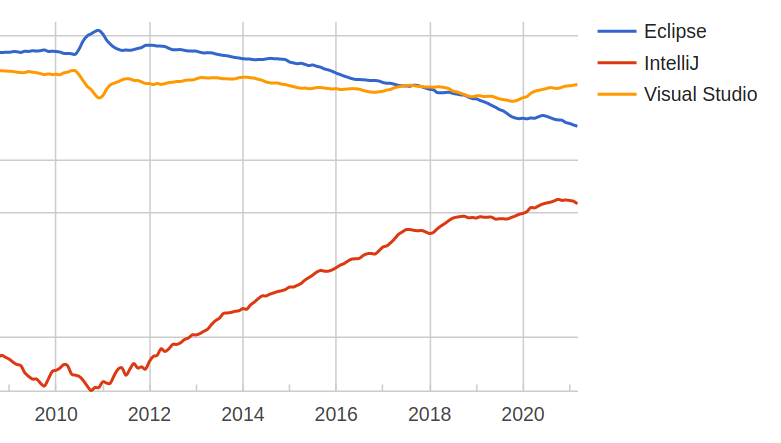
\includegraphics[width=0.8\textwidth]{images/ide-index}
	\label{img:ide-index}
\end{figure}
Aus den oben erläuterten Daten und aufgrund der guten Dokumentation für Plugin Entwicklung wird das GuttenBase als ein Intellij Plugin umgesetzt. 






\subsection{Allgemeine Beschreibung der Anforderungen}
Die Anforderungsanalyse sind mehrere Kundengespräche stattgefunden. Diese ergaben folgende Punkte, die von dem GuttenBase Plugin erfüllt werden sollen:
\begin{enumerate}
	\item \textbf{Konfigurationsschritte verwalten:}\\
	Um den Migrationsprozess zu individualisieren, soll der Benutzer die Möglichkeit haben, neue Konfigurationsschritte zu erstellen, zu editieren und zu löschen.
	\item \textbf{Konfigurationsschritte speichern:} \\
	hinugefügte Konfigurationsschritte sollen nach Bestätigung vom Benutzer gespeichert werden können. Diese sollen auch nach einem Neustart der Anwendung zur Verfügen stehen.
	\item \textbf{Überblick über alle Konsfigurationsschritte:}
	Der Benutzer soll über eine tabellarische Auflistung aller erstellten Konfigurationsschritte haben.
	\item \textbf{Datenbanken Verbiden:} \\
	Um eine erfolgreiche Migration durchzuführen, soll der Benutzer in der Lage sein, eine Verbindung zwischen der Quell- und Ziel-Datenbank herzustellen. Die zu migrierende Datenbank sowie die Ziel-Datenbank sollen aus den existierenden Datenbanken ausgewählt werden können.
	\item \textbf{Überblick über enthaltene Datenbankelemente:}\\
	Während des Pigrationsprozess, soll der Benutzer einen Überblick über alle in der Quell-Datenbank enthaltenen Tabellen bzw. Spalten verfügen.
	\item \textbf{Existierende Konfigurationsschritte zur Migration hinzufügen:}\\
	Gespeicherte Konfigurationsschritte sollen bei der Übersicht der Datenbank Elementen zur Verfügung stehen. Diese können auf die entsprechenden Datenbank Elementen angewendet werden.
	\item \textbf{Hinzugefügte Konfigurationsschritte löschen:}\\	
	Der Benutzer soll die Möglichkeit haben, hinzugefügte Konfigurationsschritte zu löschen, nachdem sie zur Migration hinzugefügt wurden.
	\item \textbf{Migrationssprozess starten:} \\
	Im letzten Schritt der Migration kann der Benutzer den Migrationsprozess mit den hinzugefügten Konfigurationsschritten starten.	
	\item \textbf{Überblick über den Fortschritt der Migrationsprozess:}\\
	Damit der Benutzer den Migrationsprozess verfolgen kann, soll einen Überblick über den Fortschritt zur verfügung stehen. 
\end{enumerate}
Konfigurationsschritte beziehen sich hauptsächlich auf die Hinweise der GuttenBase Bibliothek. Um den Umfang dieser Arbeit in Grenzen zu halten, wurden folgende wichtige Konfigurationsschritte für die Umsetzung ausgewählt:

\begin{enumerate}
	\item Spalten  umbenennen.
	\item Tabellen umbenennen.
	\item Filteroptionen für Spalten hinzufügen.
	\item Filteroptionen für Tabellen hinzufügen.
	\item Datentypen von Spalten ändern.
\end{enumerate}




\subsection{detaillierte Beschreibung der Anforderungen}
Dieser Abschnitt beschäftigt sich mit den zu implementierenden Anforderungen. Diese decken den wichtigsten Funktionsumfang des Systems.\\
Neben der textuellen Beschreibung werden auch Anwendungsfalldiagramme erstellt. Dabei wird nur ein Akteur identifiziert. Dieser ist der Benutzer, der die Datenbank Migration durchführt. \\
Um die Benutzungsführung in den Anwendungsfällen zu illustrieren und die konkrete Benutzeroberfläche, die es zu implementieren gilt, zu spezifizieren, wurden Papierprototypen für die wichtigsten Teile des Systems erzeugt. Diese basieren sich auf die Norm DIN EN ISO 9241-210.
%todo check norm


\subsubsection{Konfigurationsschritt \textbf{Unbenennen} erstellen}
	\begin{figure}[H]
		\caption{Konfigurationsschritt \glqq Unbenennen \grqq erstellen}
		\centering
		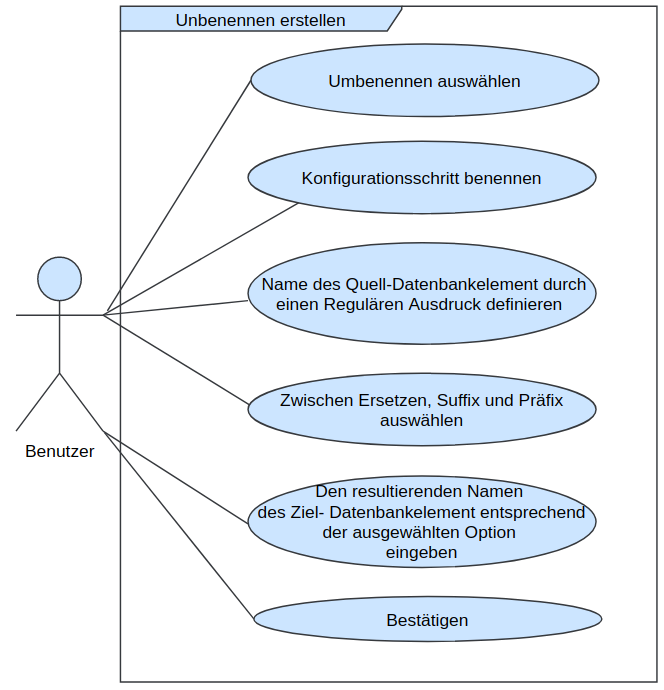
\includegraphics[width=0.7\textwidth]{images/af/af-umbenennen}
		\label{img:af-umbenennen}
	\end{figure}
Dieser Anwendungsfall bildet den Vorgang ab, wenn ein Benutzer einen neuen Konfigurationsschritt für das Umbenennen von Spalten bzw. Tabellen in der Ziel-Datenbank. Es wird vorausgesetzt, dass der Benutzer schon die Übersicht aller Konfigurationsschritte geöffnet hat (siehe Abbildung \ref{img:actions-overview}). \\
\begin{figure}[H]
	\caption{Übersicht Konfigurationsschritte}
	\centering
	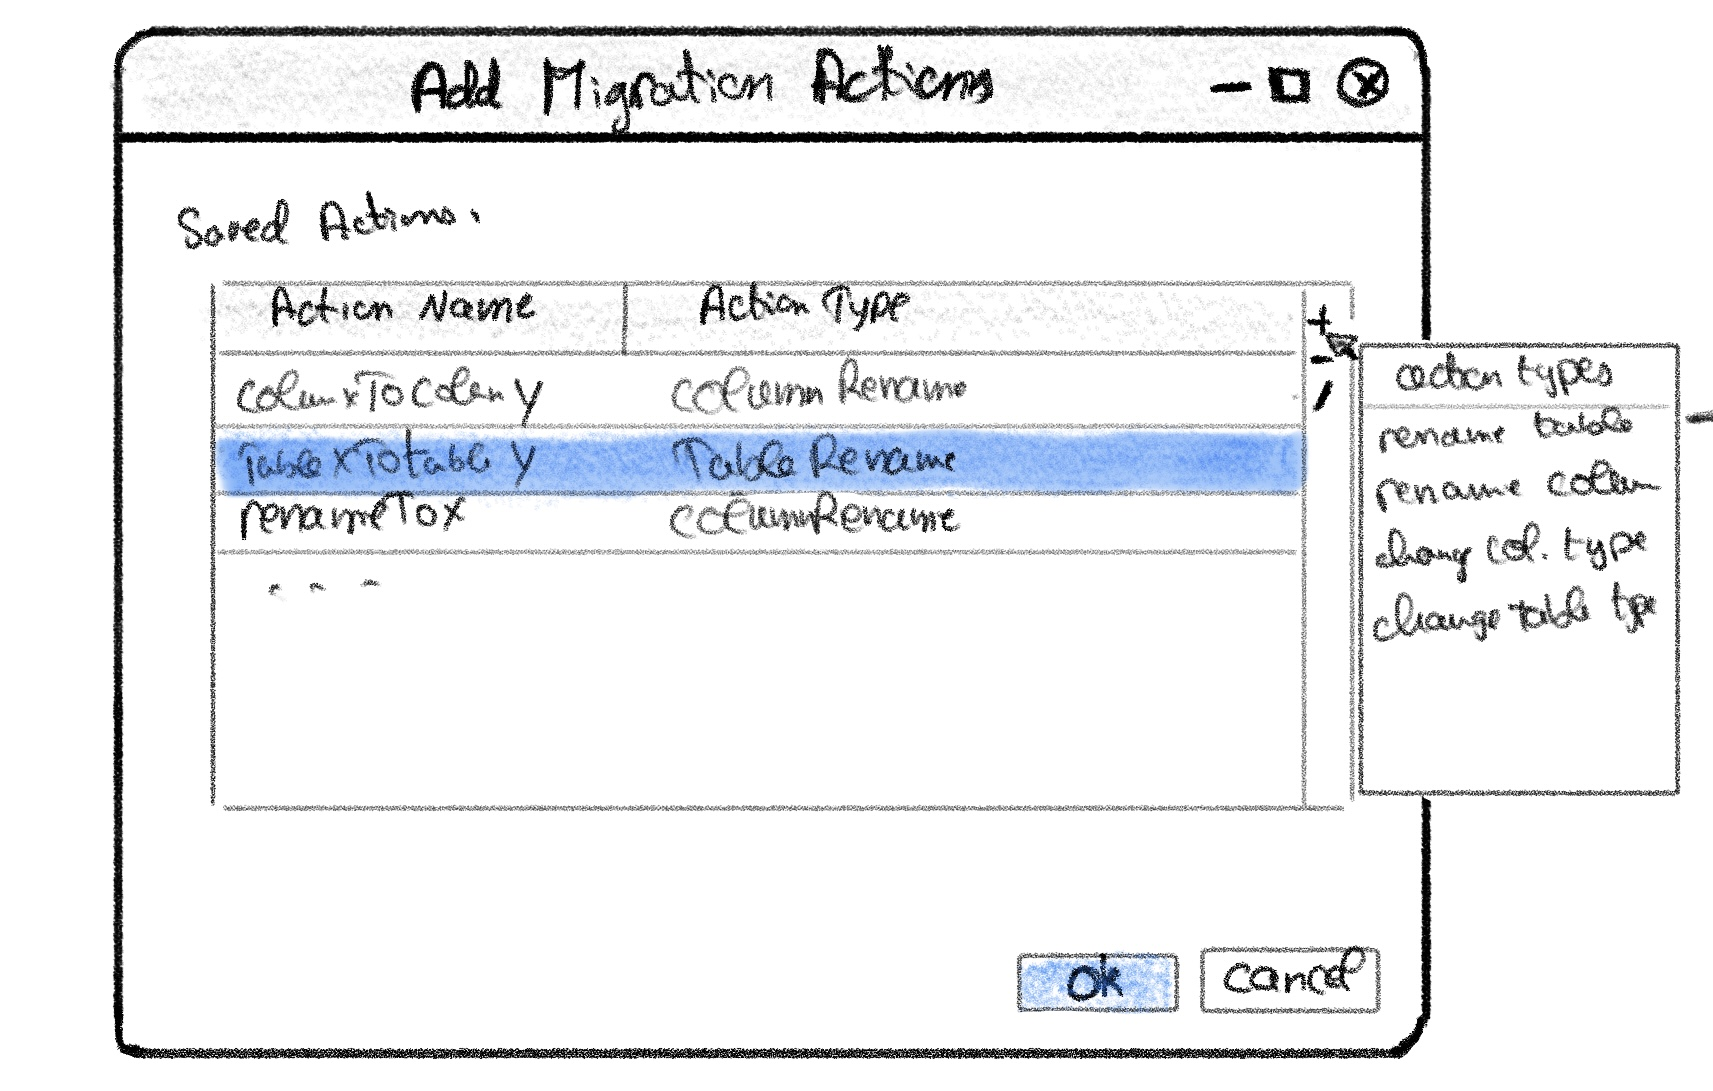
\includegraphics[width=0.5\textwidth]{images/actions-overview}
	\label{img:actions-overview}
\end{figure}
Am Anfang Soll der Benutzer den zu erstellenden Konfigurationsschritt benennen (z. B. Rename id to identifier). Das Quell-Datenbankelement (Spalte oder Tabelle) soll durch einen regulären Ausdruck definiert werden (siehe Abbildung \ref{img:add-rename-action}). Dieser wird in dem Konfigurationsschritt gespeichert, damit es später auf das Datenbank Element angewendet werden kann, das diesen Ausdruck erfüllt.
Anschließend wird der Zielname des Datenbank Elementes festgelegt. Dieser wird von dem Benutzer als eine Zeichenkette angegeben. Dabei stehen drei Optionen zur Verfügung:
\begin{itemize}
	\item \textbf{Ersetzten:} Der ganze Name des entsprechenden Datenbank Element wird durch die übergebene Zeichenkette ersetzt.
	\item \textbf{Suffix hinzufügen:} Die übergebene Zeichenkette wird als Suffix zu dem Ursprünglichen Namen hinzugefügt.
	\item \textbf{Präfix hinzufügen:} Die übergebene Zeichenkette wird als Präfix zu dem Ursprünglichen Namen hinzugefügt.
\end{itemize}
\begin{figure}[H]
	\caption{Konfigurationsschritt: Umbenennen}
	\centering
	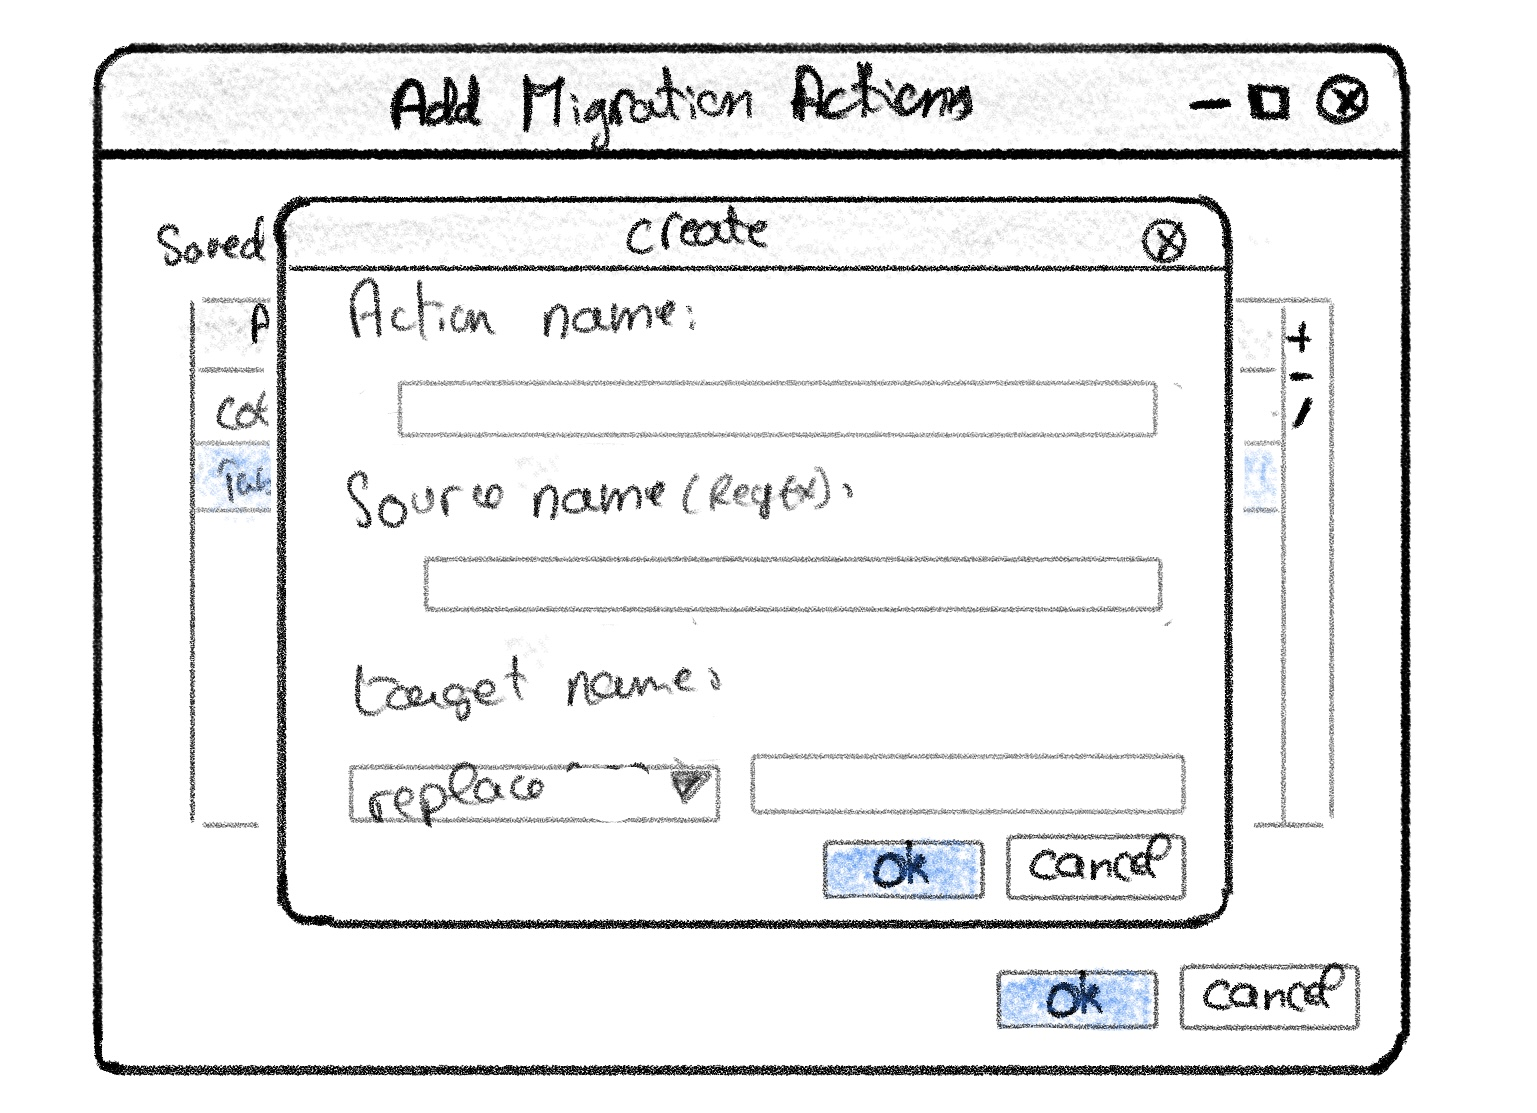
\includegraphics[width=0.5\textwidth]{images/add-rename-action}
	\label{img:add-rename-action}
\end{figure}
Nachdem Bestätigen der Eingaben wird der neu erstellten Konfigurationsschritt zu der Liste aller Konfigurationsschritten hinzugefügt.

\begin{table}[H]
	\centering
	\begin{tabular}{ |p{4cm}|p{8cm}| }
		\hline
		\textbf{Name} &  Konfigurationsschritt Unbenennen erstellen \\
		\hline
		\textbf{Akteure} & Benutzer \\
		\hline
		\textbf{Auslöser} & Der Nutzer ist bei der übersicht der Konfigurationsschritte und hat auf das \glqq $+$\grqq Button geklickt. \\
		\hline
		\textbf{Vorbedingung} & Der Nutzer besitzt eine List von Konfigurationsschritten.  \\
		\hline
		\textbf{Nachbedingung} & Ein Konfigurationsschritt vom Typ Umbenennen wird zur Liste aller Konfigurationsschritte hinzugefügt.  \\
		\hline
		\textbf{Ablauf} & 
		\begin{enumerate}
			\item Die Option \glqq Umbenennen\grqq auswählen.
			\item Einen Namen für den zu erstellenden Konfigurationsschritt eingeben.
			\item Den Namen des Quell-Datenbankelement durch einen regulären Ausdruck definieren.
			\item Zwischen Ersetzen, Suffix und Präfix auswählen.
			\item Den resultierenden Namen des Ziel- Datenbankelement entsprechend der ausgewählten Option eingeben.
			\item Bestätigen.
		\end{enumerate}  \\
		\hline
		
	\end{tabular}
	\caption{Anwendungsfall Konfigurationsschritt \textbf{Unbenennen} erstellen}
	\label{table:umbenennen}
\end{table}




\subsubsection{Konfigurationsschritt \textbf{Datentyp Ändern} erstellen}
\begin{figure}[H]
	\caption{Konfigurationsschritt \glqq Datentyp Ändern \grqq erstellen}
	\centering
	\includegraphics[width=0.7\textwidth]{images/af/af-datentyp-ändern}
	\label{img:af-datentyp-ändern}
\end{figure}
Dieser Anwendungsfall zeigt, wie der Benutzer den Konfigurationsschritt \textbf{Datentyp Ändern} erstellt. Wie der vorherige Anwendungsfall soll der Benutzer bei der Übersicht aller Konfigurationsschritte sein, um in den Anwendungsfall einzutreten (siehe Abbildung \ref{img:actions-overview}).\\
Nach dem Auslösen des Anwendungsfalls soll der Benutzer die Option \glqq Datentyp Ändern\grqq auswählen. Danach hat der Benutzer die Mööglichkeit, den Konfigurationsschritt zu benennen, den Datentyp der Quell-Datenbank bzw. der Ziel-Datenbank als Zeichenkette einzugeben und anschließend die Eingaben bestätigen. Nachdem dieser Anwendungsfall beendet ist, wird ein neuer Konfigurationsschritt hinzugefügt.\\ \\
Das Erstellen vom Konfigurationsschritt \glqq Excludieren \grqq läuft im Grunde ähnlich ab, wie die zwei vorherigen Anwendungsfälle und wird daher nicht behandelt.
\begin{table}[H]
	\centering
	\begin{tabular}{ |p{4cm}|p{8cm}| }
		\hline
		\textbf{Name} &  Konfigurationsschritt Datentyp Ändern erstellen \\
		\hline
		\textbf{Akteure} & Benutzer  \\
		\hline
		\textbf{Auslöser} & Der Nutzer ist bei der übersicht der Konfigurationsschritte und hat auf das \glqq $+$\grqq Button geklickt.  \\
		\hline
		\textbf{Vorbedingung} & Der Nutzer besitzt eine List von Konfigurationsschritten.  \\
		\hline
		\textbf{Nachbedingung} & Ein Konfigurationsschritt vom Typ Datentyp Ändern wird zur Liste aller Konfigurationsschritte hinzugefügt.  \\
		\hline
		\textbf{Ablauf} & 
		\begin{enumerate}
			\item Die Option \glqq Datentyp Ändern\grqq auswählen.
			\item Einen Namen für den zu erstellenden Konfigurationsschritt eingeben.
			\item Den Datentyp des Quell-Spalte festlegen.
			\item Den Datentyp des Ziel-Spalte eingeben.
			\item Bestätigen.
		\end{enumerate}   \\
		\hline
		
	\end{tabular}
	\caption{Anwendungsfall Konfigurationsschritt \textbf{Datentyp Ändern} erstellen}
	\label{table:datentyp-ändern}
\end{table}




\subsubsection{Konfigurationsschritte verwalten}
\begin{figure}[H]
	\caption{Konfigurationsschritte verwalten}
	\centering
	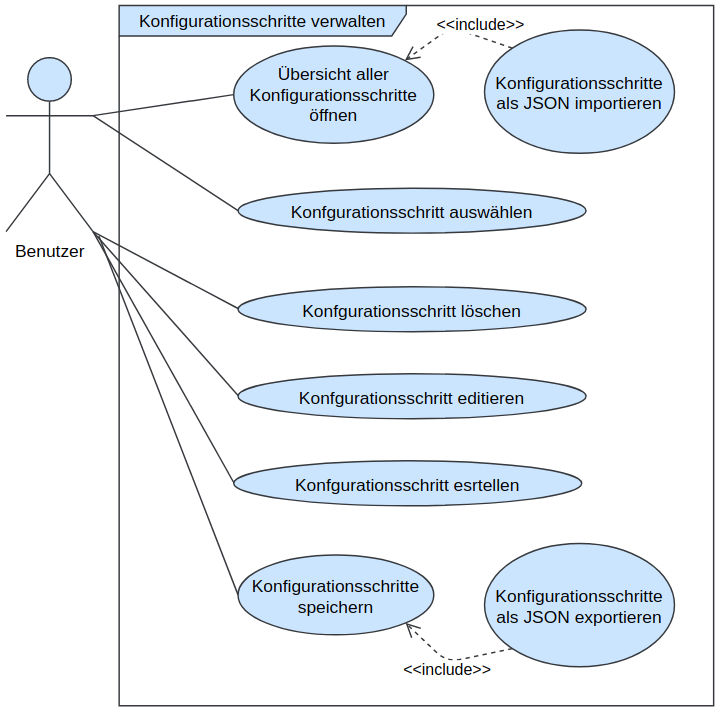
\includegraphics[width=0.7\textwidth]{images/af/af-ks-verwalten}
	\label{img:af-ks-verwalten}
\end{figure}
Dieser Anwendungsfall stellt die Verwaltung der Konfigurationsschritte dar. Als erstes soll der Benutzer die Übersicht der Konfigurationsschritte öffnen (siehe Abbildung \ref{img:actions-overview}). Dabei werden alle gespeicherten Konfigurationsschritte geladen. Diese werden aus einer JSON Datei erzeugt. \\
Bei der Übersicht kann der Benutzer einzelne oder mehrere Konfigurationsschritte auf einmal löschen. Außerdem kann der Benutzer Konfigurationsschritte erstellen (Diese wurde in den vorherigen Anwendungsfällen beschrieben). Das Editieren der Konfigurationsschritte erfolgt genauso wie das Erstellen.\\
Anschließend können Konfigurationsschritte, nach Bestätigung vom Benutzer, als JSON gespeichert werden.
\begin{table}[H]
	\centering
	\begin{tabular}{ |p{4cm}|p{8cm}| }
		\hline
		\textbf{Name} & Konfigurationsschritte verwalten  \\
		\hline
		\textbf{Akteure} &  Benutzer \\
		\hline
		\textbf{Auslöser} &  Der Benutzer klickt auf ein Button, um die Übersicht aller Konfigurationsschritte zu sehen. \\
		\hline
		\textbf{Vorbedingung} & Der Benutzer hat eine initiale List von Konfigurationsschritten.  \\
		\hline
		\textbf{Nachbedingung} & Änderungen sind vorgenommen und gespeichert.  \\
		\hline
		\textbf{Ablauf} & 
		\begin{enumerate}
			\item Übersicht aller Konfigurationsschritte öffnen.
			\item eventuell Konfgurationsschritte auswählen.
			\item eventuell Konfgurationsschritte löschen.
			\item eventuell einen Konfgurationsschritt editieren.
			\item eventuell einen Konfgurationsschritt esrtellen.
			\item Konfigurationsschritte speichern.
		\end{enumerate}   \\
		\hline
		
	\end{tabular}
	\caption{Anwendungsfall Konfigurationsschritte verwalten}
	\label{table:ks-speichern}
\end{table}



\subsubsection{Datenbank Migration durchführen}
Das Durchführen der Datenbank Migraion deckt die Hauptfunktionalität des GuttenBase Plugins ab. Dies wird in folgenden Anwendungsfällen unterteilt: 
	\subsubsection*{Datenbanken verbinden}
	\begin{figure}[H]
		\caption{Datenbanken verbinden}
		\centering
		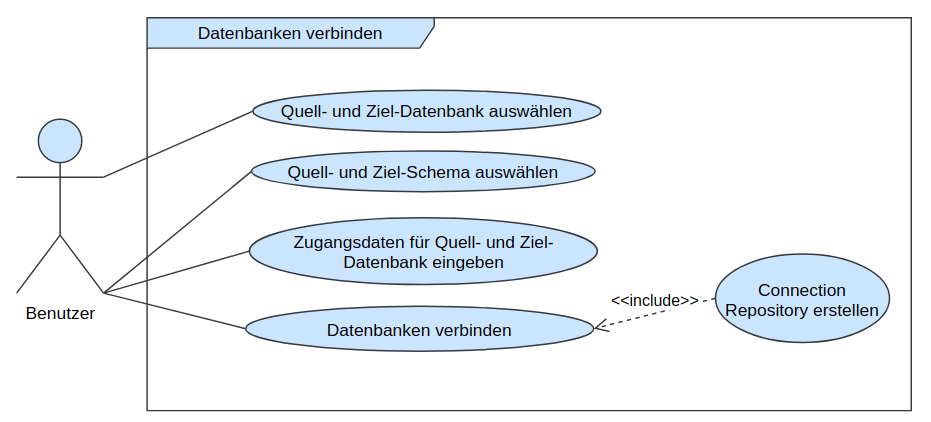
\includegraphics[width=0.7\textwidth]{images/af/af-db-verbinden}
		\label{img:af-db-verbinden}
	\end{figure}
	Für das Eintreten dieses Anwendungsfalls is vorausgesetzt, dass der Benutzer über mindestens eine Datenbank verfügen. Am Anfang soll der Benutzer das Migrationsfenster öffnen um die Eingabefelder zu sehen. Zunächst soll der Benutzer die Datenbank, das Schema, die Zugangsdaten für das Quell- und Ziel-DBMS (siehe Abbildung \ref{img:generalview}).
	Wenn die Eingaben stimmen, kann der Benutzer eine Verbingung zwischen den beiden Datenbanken herstellen. Ansonsten soll eine Entsprechende Meldung angezeigt werden. Bei diesem Schritt wird der Connector Repository der GuttenBase Bibliothek erstellt und konfiguriert. Somit ist die Datenbank Migration bereit für die Konfiguration.
	\begin{figure}[H]
		\caption{Datenbank Migration View}
		\centering
		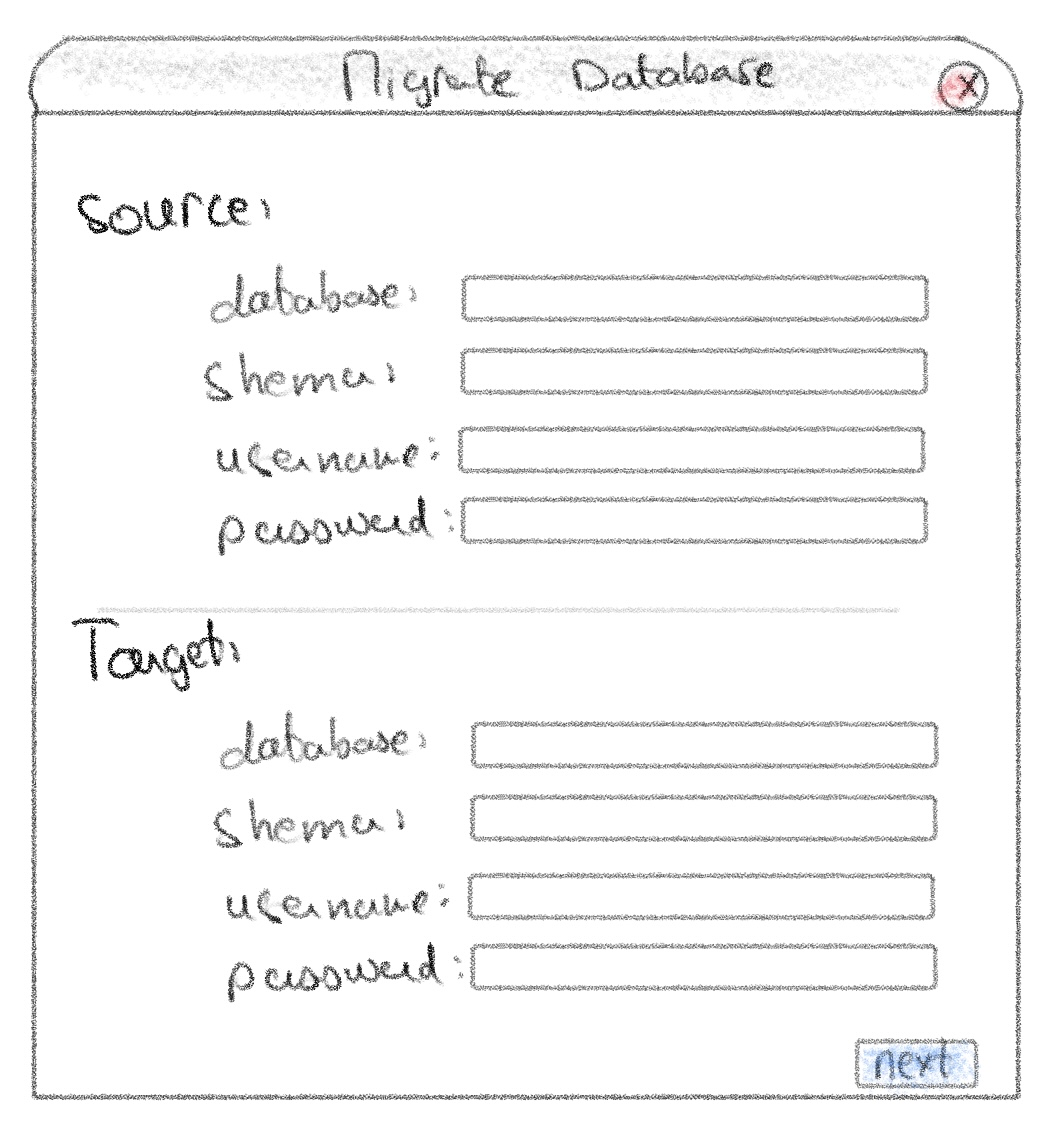
\includegraphics[width=0.5\textwidth]{images/generalview}
		\label{img:generalview}
	\end{figure}
	\begin{table}[H]
		\centering
		\begin{tabular}{ |p{4cm}|p{8cm}| }
			\hline
			\textbf{Name} & Datenbanken verbinden  \\
			\hline
			\textbf{Akteure} & Benutzer  \\
			\hline
			\textbf{Auslöser} & Der Benutzer klickt auf ein Button um die Übersicht der Datenbankverbindung zu öffnen. \\
			\hline
			\textbf{Vorbedingung} &  Quell- und Ziel-Datenbanken sind nicht mit dem GuttenBase Tool verbunden.\\
			\hline
			\textbf{Nachbedingung} & Quell- und Ziel-Datenbanken sind verbunden.  \\
			\hline
			\textbf{Ablauf} &  
			\begin{enumerate}
				\item Quell-Datenbank auswählen.
				\item Quell-Schema auswählen.
				\item Benutzername der Quell-Datenbank eingeben.
				\item Passwort der Quell-Datenbank eingeben.
				\item Ziel-Datenbank auswählen.
				\item Ziel-Schema auswählen.
				\item Benutzername der Ziel-Datenbank eingeben.
				\item Passwort der Ziel-Datenbank eingeben.
				\item Datenbanken verbinden
			\end{enumerate}  \\
			\hline
			
		\end{tabular}
		\caption{Anwendungsfall Datenbanken verbinden}
		\label{table:db-verbinden}
	\end{table}
		
		
	\subsubsection*{Migrationsprozess konfigurieren}
	\begin{figure}[H]
		\caption{Migrationsprozess konfigurieren}
		\centering
		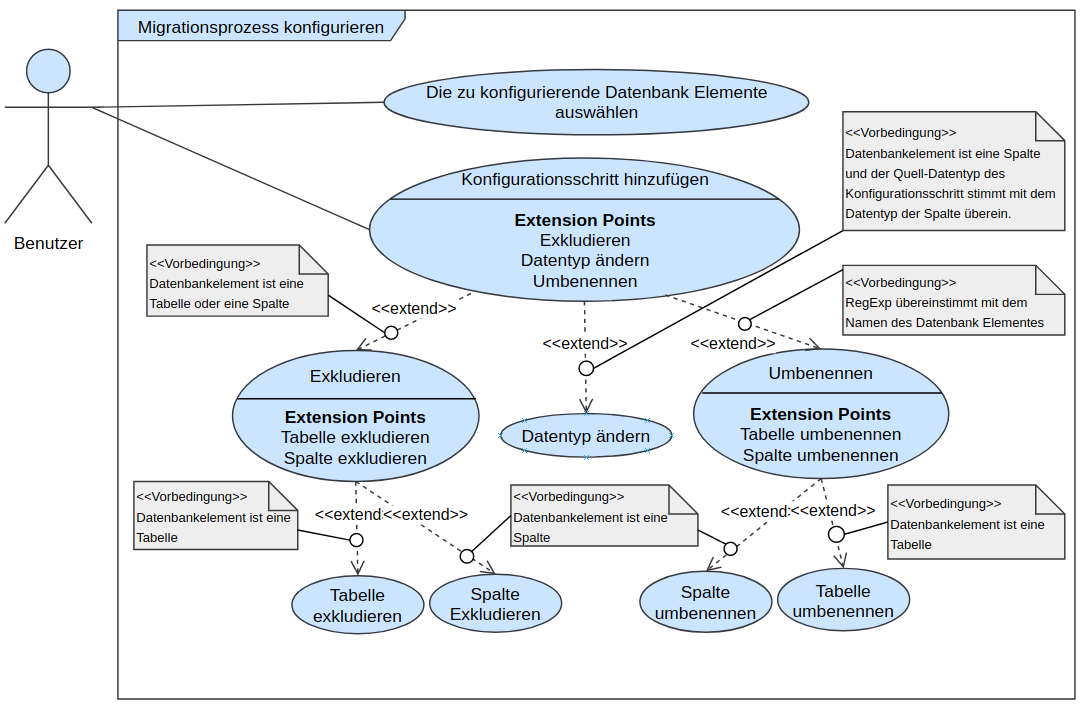
\includegraphics[width=0.9\textwidth]{images/af/af-mg-cfg}
		\label{img:af-mg-cfg}
	\end{figure}
	Dieser Anwendungsfall bildet den Vorgang ab, wie der Benutzer Konfigurationsschritte zum Migrationsprozess hinzufügt.\\
	Es wird vorausgesetzt, dass die Quell- und Ziel-Datenbanken verbuden sind. (siehe Anwendungsfall \ref{table:db-verbinden})\\
	Wenn der Nutzer auf das \glqq Next\grqq geklickt hat, soll eine Übersicht für alle in der Quell-Datenbank enthaltenen Elemente angezeigt werden (Siehe Abbildung \ref{img:overview}).
	\begin{figure}[H]
		\caption{Übersicht Quell-Datenbank}
		\centering
		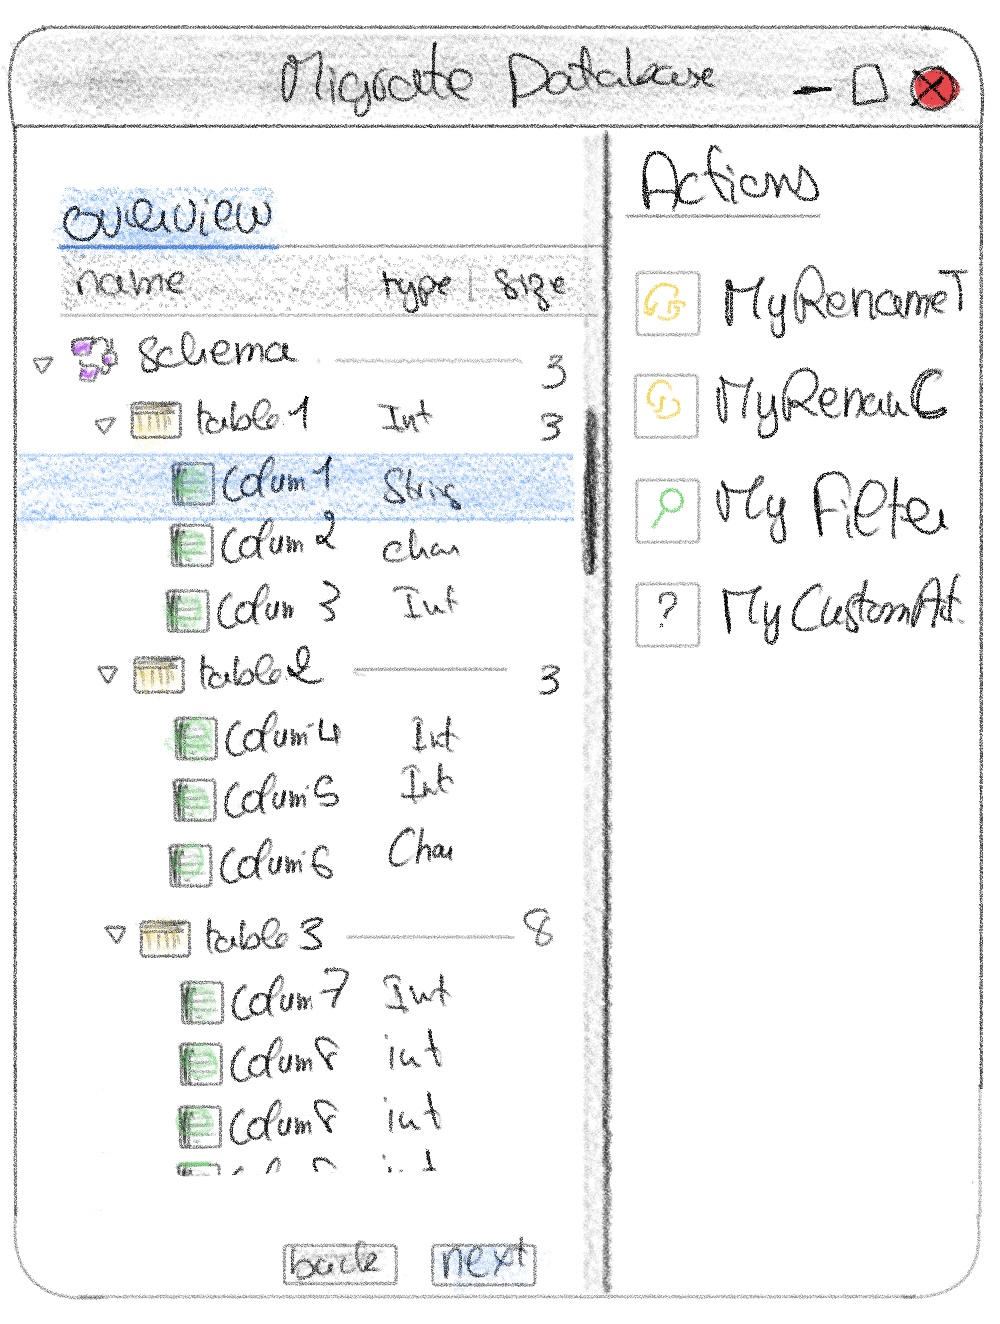
\includegraphics[width=0.5\textwidth]{images/overview}
		\label{img:overview}
	\end{figure}
	Der Benutzer kann zunächst Spalten bzw. Tabellen auswählen, um denen Konfigurationsschritte zuzuweisen.\\
	Jenachdem wie die Auswahl der Datenbankelemente aussieht, stehen nur die passenden Konfigurationsschritte zur Verfügung. Um eine Tabelle bzw. eine Spalte zu exkludieren, reicht es wenn das selektierte Datenbankelement eine Tabelle bzw. eine Spalte ist. \\
	Auf der anderen Seite wird beim Hinzufügen des Konfigurationsschritts \glqq DatenTyp ändern \grqq geprüft, ob die ausgewählten Datenbankelemente Spalten sind und ob deren Datentypen dem Datentyp des Konfigurationsschrittes entsprechen. \\
	Außerdem wird beim Umbenennen der ausgewählten Tabellen bzw Spalten geprüft, ob die Namen mit dem im Konfigurationsschritt gespeicherten regulären Ausdruck übereinstimmen.\\
	Nachdem der Benutzer alle gewünschte Konfigurationsschritte hinzugefügt hat, werden diese gemerkt und zu dem Migrationsprozess hinzugefügt.
		\begin{table}[H]
		\centering
		\begin{tabular}{ |p{4cm}|p{8cm}| }
			\hline
			\textbf{Name} &  Migrationsprozess konfigurieren. \\
			\hline
			\textbf{Akteure} & Benutzer  \\
			\hline
			\textbf{Auslöser} & Der Benutzer klickt auf das \glqq Next\grqq Button.  \\
			\hline
			\textbf{Vorbedingung} &  Die Migration ist nicht konfiguriert. \\
			\hline
			\textbf{Nachbedingung} &  Die Migration ist nach den Wünschen des Benutzers konfiguriert. \\
			\hline
			\textbf{Ablauf} & 
			\begin{enumerate}
				\item Die zu konfigurierende Datenbank Elemente auswählen.
				\item Konfigurationsschritt hinzufügen (Dieser Schritt kann mehrmals durchgeführt werden).
			\end{enumerate}   \\
			\hline
			
		\end{tabular}
		\caption{Anwendungsfall Migrationsprozess konfigurieren}
		\label{table:migration-cfg}
	\end{table}



	\subsubsection*{Hinzugefügte Konfigurationsschritte löschen}	
	\begin{figure}[H]
		\caption{Hinzugefügte Konfigurationsschritte löschen}
		\centering
		\includegraphics[width=0.7\textwidth]{images/af/af-ks-löschen}
		\label{img:af-ks-löschen}
	\end{figure}
	Das Löschen eines hinzugefügten Konfigurationsschritt ist erst möglich, wenn der Benutzer in der entsprechenden Übersicht ist (siehe Abbildung \ref{img:result-view}). Dabei werden alle hinzugefügten Konfigurationsschritte aufgelistet.Diese können ausgewählt und anschlißend gelöscht werden.
	\begin{figure}[H]
		\caption{Übersicht hinzugefügte Konfigurationsschritte}
		\centering
		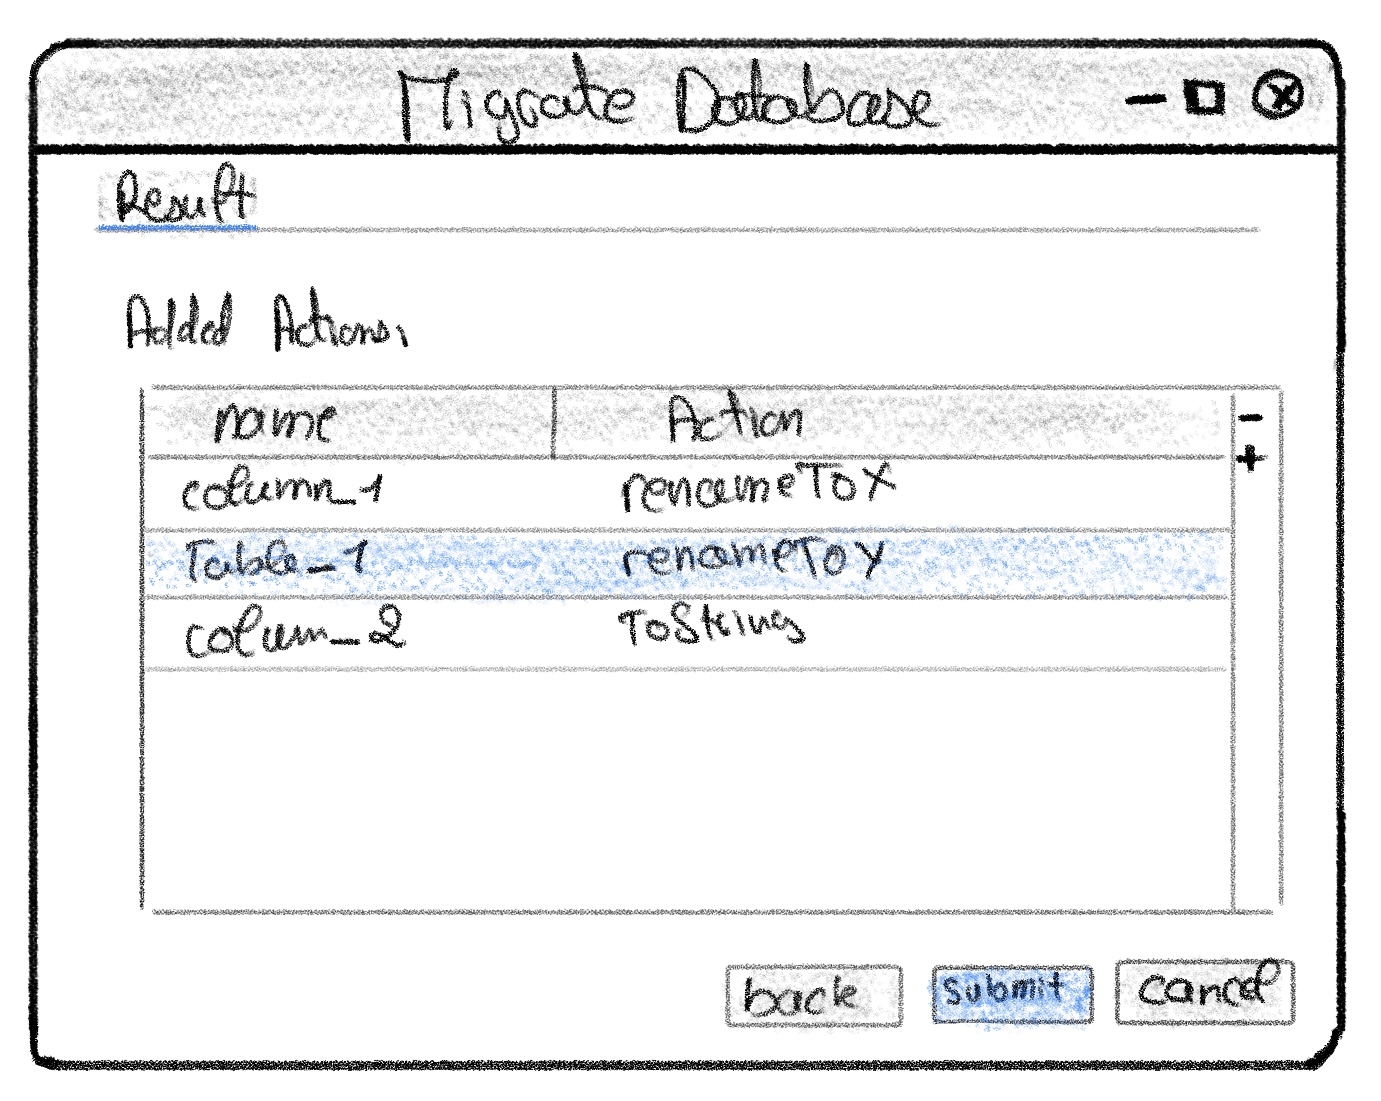
\includegraphics[width=0.6\textwidth]{images/result-view}
		\label{img:result-view}
	\end{figure}
		\begin{table}[H]
		\centering
		\begin{tabular}{ |p{4cm}|p{8cm}| }
			\hline
			\textbf{Name} &  Hinzugefügte Konfigurationsschritte löschen \\
			\hline
			\textbf{Akteure} &  Benutzer \\
			\hline
			\textbf{Auslöser} & Der Benutzer klickt auf das \glqq Next\grqq Button.  \\
			\hline
			\textbf{Vorbedingung} &   \\
			\hline
			\textbf{Nachbedingung} &   \\
			\hline
			\textbf{Ablauf} &  
			\begin{enumerate}
				\item Die zu löschende Konfigurationsschritte auswählen.
				\item Ausgewählte Konfigurationsschritt löschen.
			\end{enumerate}  \\
			\hline
			
		\end{tabular}
		\caption{Anwendungsfall Hinzugefügte Konfigurationsschritte löschen}
		\label{table:migration-ks-löschen}
	\end{table}



	\subsubsection*{Migration starten}
	\begin{figure}[H]
		\caption{Migration starten}
		\centering
		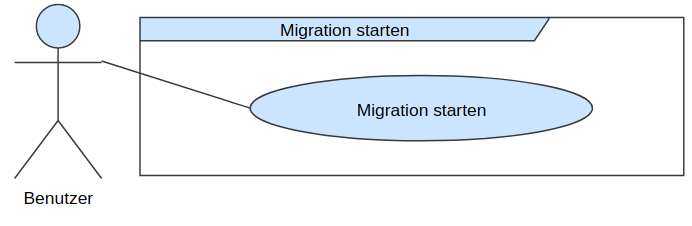
\includegraphics[width=0.7\textwidth]{images/af/af-mg-starten}
		\label{img:af-mg-starten}
	\end{figure}
	Nachdem der Benutzer alle die Datenbanken verbunden und den Migrationsprozess konfiguriert hat, kann er die Migration der Datenbank durch eine einfache Bestätigung starten. Danach sollen die Daten entsprechend der Konfiguration migriert werden. Währenddessen soll der Benutzer über den Migrationsstand informiert werden (siehe Abbildung \ref{img:progressview}).
	\begin{figure}[H]
		\caption{Fortschritt vom Migrationsprozess}
		\centering
		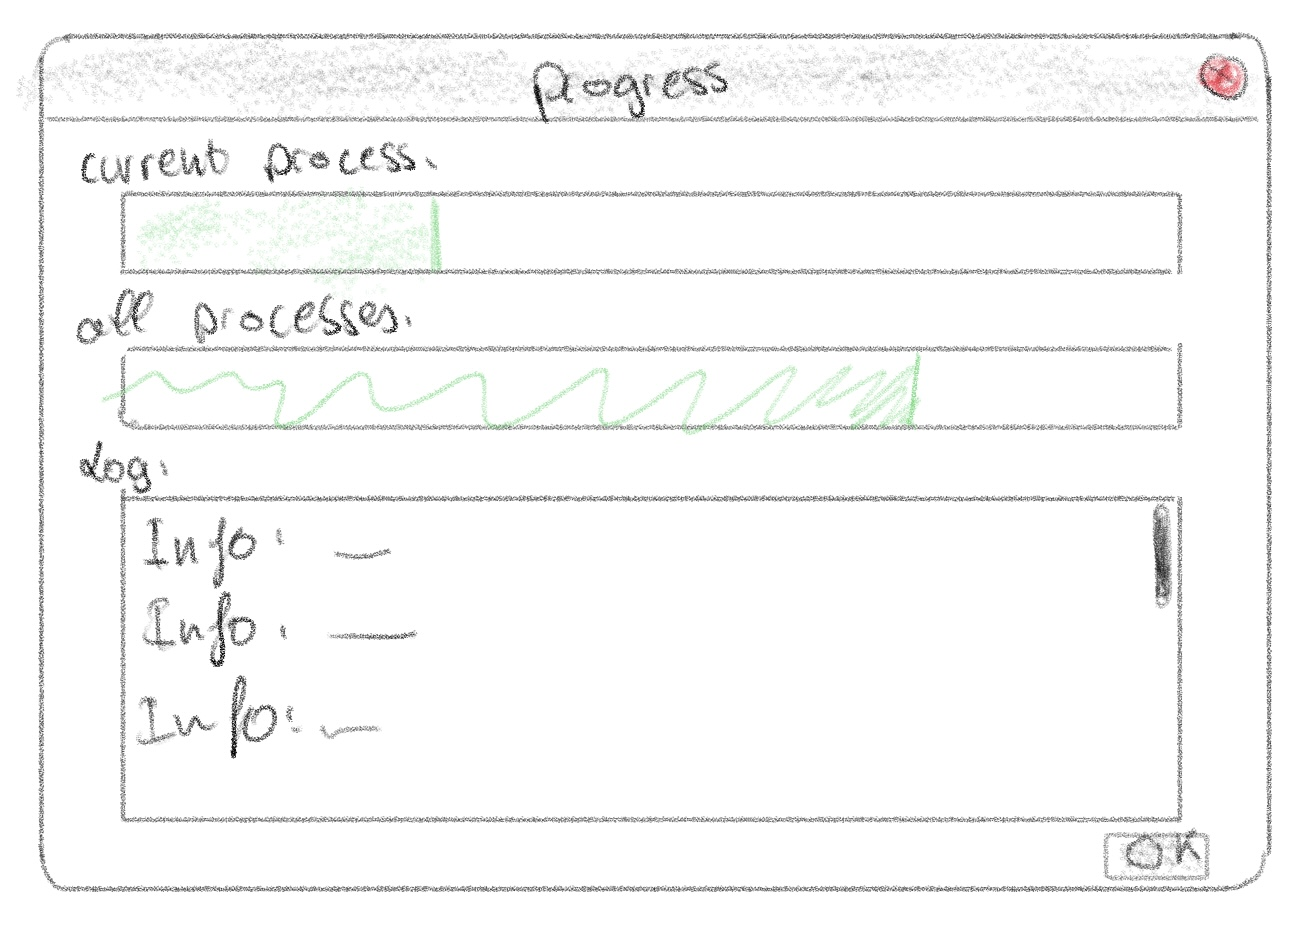
\includegraphics[width=0.4\textwidth]{images/progressview}
		\label{img:progressview}
	\end{figure}
			\begin{table}[H]
		\centering
		\begin{tabular}{ |p{4cm}|p{8cm}| }
			\hline
			\textbf{Name} & Migration starten  \\
			\hline
			\textbf{Akteure} & Benutzer  \\
			\hline
			\textbf{Auslöser} & Der Benutzer klickt auf das \glqq Migrieren\grqq Button.  \\
			\hline
			\textbf{Vorbedingung} & Quell-Datenbank ist noch nicht migriert.  \\
			\hline
			\textbf{Nachbedingung} & Quell-Datenbank ist migriert.  \\
			\hline
			\textbf{Ablauf} &  
			\begin{enumerate}
				\item Migration starten.
			\end{enumerate}  \\
			\hline
			
		\end{tabular}
		\caption{Anwendungsfall Migration starten}
		\label{table:migration-starten}
	\end{table}

\subsection{Datensicht}
%\subsection{Probleme und Strategien}
%- Umsetzungsform\\
%- ...
\section{Konzeption}
%- DatenModell: GBActions, DB Elemente\\
%- Abstrakte Mapping \\
%- Multiple Select \\
%- Aktionen speichern \\
%- Protoypen \\
%- allgemeines: warum muss erst die Umsetzungsform entschieden werden (vor der Konzeption). \\
%- welche Alternativen gibt es um ein solches Plugin entwickeln zu können?\\
%- Vorteile und Nachteile jeder Alternative.\\
%- Argumente für IntelliJ Plugin.
%- Was ist IntelliJ \\
%- was ist IntelliJ Plugin Entwicklung \\
%- wie lässt sich ein Plugin mit IntelliJ entwickeln?\\

\subsection{Konzeptionelle Sicht}
\subsection{Modulsicht}



\section{Implementierung}
\subsection{verwendete Technologien}
- Swing \\
- UI Form \\
- Java\\
- Gutenbase
\subsubsection{IntelliJ Plugin Entwicklung}

\subsection{Features}
%- add gbact\\
%- save gb act\\
%- migrate db \\
%- + screenshots usw.


